% DI Atlas paper — v5, formatted for PLOS Computational Biology
% Batch 3 (F, G, H): MoA stratification, cross-cell-line CRISPR pilot, DepMap
% convergent failure.

\documentclass[11pt]{article}

\usepackage{amsmath,amssymb}
\usepackage{booktabs}
\usepackage{array}
\usepackage{graphicx}
\usepackage[hyphens]{url}
\usepackage{hyperref}
\usepackage[margin=1in]{geometry}
\usepackage[numbers,sort&compress]{natbib}
\usepackage{xcolor}
\usepackage{multirow}
\usepackage[affil-it]{authblk}

\renewcommand{\arraystretch}{1.3}

\title{An Atlas of Cross-Context Consistency\\
for 55,000 Drug and Genetic Perturbations}

\author{Elliot Tower}
\affil{Independent researcher \\ \texttt{elliot@elliottower.ai}}
\date{}

\begin{document}
\maketitle

\begin{abstract}
Direction instability (DI) measures whether a perturbation's effects point the
same way across contexts, as the mean pairwise cosine dissimilarity among its
signatures.  DI is the complement of pairwise phase consistency, applied
here at atlas scale: magnitude-corrected, with
bootstrap confidence intervals, across ${\sim}$55{,}000 drug and genetic
perturbations drawn from LINCS L1000, Tahoe-100M, and the JUMP Cell Painting (JUMP-CP)
compound, CRISPR, and ORF datasets.

Eleven hypotheses were pre-registered across three batches before computation.
Two met their pre-registered criteria, eight failed, and one gave directional
exploratory support. The failures are what constrain the metric:
knockout and overexpression DI for the same gene are unrelated
($\rho = 0.011$, $n = 5{,}220$), and expression variance, paralog count, and
paralog expression breadth each explain under 0.4\% of DI variance after
confound control.  The principal positive result is that drug
mechanism-of-action class explains 20\% of residualized DI variance
($\eta^2 = 0.201$, permutation $p < 0.001$), separating core-machinery
inhibitors (mTOR, HDAC; low~DI) from receptor-signaling drugs (serotonin and
histamine agonists; high~DI).

DI computed over JUMP-CP plate replicates indexes technical reproducibility
within a single cell line rather than context-dependence across cell types.
On those values, essentiality breadth predicts \emph{lower} DI---the opposite
of the registered prediction---at partial $\rho = -0.332$, attenuating to
$\rho = -0.189$ when signal strength is also controlled; the direction
replicates on a two-cell-line CRISPR pilot ($\rho = -0.264$, $n = 128$).  The
atlas is released as a resource, with per-perturbation DI values, confidence
intervals, analysis code, and the frozen pre-registration record.
\end{abstract}


%% ====================================================================
\section{Introduction}
%% ====================================================================

High-throughput perturbation screens now profile thousands of drugs and
genetic perturbations across panels of cell lines, producing
multi-dimensional signatures in transcriptomic
\citep{lamb2006connectivity, subramanian2017next}, morphological
\citep{bray2016cell}, and single-cell modalities \citep{tahoe2025}.  Three
resources recur throughout: LINCS L1000 (Library of Integrated Network-Based
Cellular Signatures, a transcriptomic screen reporting 978 landmark genes),
JUMP-CP (Joint Undertaking in Morphological Profiling---Cell Painting, an
image-based morphological screen), and Tahoe-100M (a single-cell
transcriptomic perturbation atlas).
Whether a perturbation's effects transfer across cellular contexts has
practical consequences for drug development and genetic screening
\citep{mcfarland2020context, tower2026confound}.

Direction instability (DI) quantifies this context-dependence as
$\mathrm{DI} = 1 - \overline{\cos(\mathbf{s}_i, \mathbf{s}_j)}$, the
mean pairwise cosine dissimilarity among a perturbation's signatures
across contexts.

This quantity is not new.  Writing $\bar{R} = \|\sum_i \mathbf{u}_i\|/K$ for
the mean resultant length of the unit-normalized signatures,
Equation~\ref{eq:di} is $\frac{K}{K-1}(1 - \bar{R}^2)$, and the mean pairwise
cosine is $(K\bar{R}^2 - 1)/(K-1)$.  The latter is pairwise phase consistency
(PPC), introduced by \citet{vinck2010ppc} as a bias-free measure of
synchronization---so $\mathrm{DI} = 1 - \mathrm{PPC}$.  PPC was designed for
exactly the property claimed here, separating consistency from apparent
strength due to sample size.  What this study contributes is therefore not the
statistic but its application: perturbation-specific, computed across cell
lines, magnitude-corrected, and at atlas scale, against a panel of public
perturbation datasets that PPC has not been applied to.  Related work on
perturbation coherence is discussed in Section~\ref{sec:discussion}.

DI complements rather than replaces the perturbation-quality and retrieval
metrics already in use on these datasets, and the estimands differ.  The L1000
Transcriptional Activity Score combines signature strength with replicate
concordance to identify transcriptionally active perturbations, so it is
designed to register the conjunction that DI separates.  Cell Painting
percent-replicating asks whether replicate profiles are more similar to each
other than a null distribution allows, and mean average precision scores
retrieval of known replicate or annotation groups.  Each of these answers
whether a perturbation produced a reproducible measurable signal, or how well
profiles retrieve a stated label.  DI answers a different question: given that a
signal is present, how much does its direction change across the contexts the
analyst designates.  A perturbation can score well on activity and retrieval
while carrying high DI, and the reverse holds for a weak but directionally
stable perturbation.  Concurrent work on geometric stability
\citep{raju2026a, raju2026b} measures perturbation coherence on a related axis;
it aggregates over individual cells within one context, whereas DI aggregates
across the contexts an analyst designates, so the two quantify different
variation and are not interchangeable.  Because cosine normalizes each signature to unit
length before comparison, DI is immune to the first-order magnitude
confound---systematic covariation between effect size and metric
value---that dominates alternative geometric measures such as
Grassmannian geodesic distance, profile variability, and optimal
transport cost \citep{tower2026confound}.  A residual second-order
correlation persists near zero (noise-dominated signatures inflate
pairwise cosine dissimilarity), which we remove by magnitude correction
(Section~\ref{sec:atlas}).  A companion study \citep{tower2026confound}, a preprint under peer review,
reports this immunity.  In leave-one-cell-line-out analysis of 2{,}694 drugs
profiled in at least ten cell lines, DI predicted a cosine-defined held-out
consistency outcome with AUROC $= 0.986$ before and $0.864$ after magnitude
correction.  Predictor and outcome share cosine geometry, and a geometry-matched
synthetic null in that study reaches AUROC $= 0.996$, above the value obtained on
real drugs; the held-out prediction therefore characterizes out-of-sample
geometric consistency rather than validating biological transport.  The
biological evidence comes instead from criteria that do not involve cosine
similarity: Jaccard overlap of held-out top gene sets (AUROC $= 0.957$), breadth
of target gene expression across tissues in CCLE ($\rho = -0.170$,
$p = 1.1 \times 10^{-5}$), and PRISM cell-viability variability
($\rho = 0.261$, $p = 0.019$).  That study is a preprint under
peer review rather than published work, so its headline evidence is reproduced
here (Table~\ref{tab:companion}) and this manuscript does not rest on it.  Sections that depend on it are
marked at the point of use.  The present study asks a different question: what does DI capture, and what does it fail to capture, across
modalities and perturbation types?

\vspace{1em}
\begin{table}[htbp]
\centering
\caption{Validation evidence for DI reported in the companion study, reproduced
here so this manuscript can be read on its own.  The first row is a geometric
characterization rather than biological validation: predictor and outcome share
cosine geometry, and a geometry-matched synthetic null reaches AUROC $= 0.996$ in
that study, above the value obtained on real drugs.  The remaining three rows do
not involve cosine similarity, and the last two are measured on external
datasets.  The held-out cosine analysis covers 2{,}694 drugs profiled in at
least ten cell lines; the gene-set criterion is computed on LINCS signatures.
The companion study is a preprint under peer review at the time of writing.}
\label{tab:companion}
\small
\begin{tabular}{@{}llr@{}}
\toprule
\textbf{Channel} & \textbf{Criterion} & \textbf{Effect} \\
\midrule
Held-out cosine & Leave-one-cell-line-out consistency & AUROC $= 0.986$ raw, $0.864$ corrected \\
Gene-set & Jaccard overlap of held-out top genes & AUROC $= 0.957$ \\
Expression & CCLE target-gene breadth across tissues & $\rho = -0.170$, $p = 1.1 \times 10^{-5}$ \\
Viability & PRISM cell-viability variability & $\rho = 0.261$, $p = 0.019$ \\
\bottomrule
\end{tabular}
\end{table}

We constructed a DI atlas spanning three measurement technologies and
four perturbation classes: drug perturbations measured by L1000
transcriptomics (LINCS, 8{,}949 compounds) and single-cell
transcriptomics (Tahoe-100M, 379 compounds); genetic knockouts measured
by Cell Painting morphology (JUMP-CP CRISPR, 7{,}946 genes); and
genetic overexpressions measured by Cell Painting morphology (JUMP-CP
ORF, 12{,}590 genes).  For each perturbation, the atlas provides
magnitude-corrected DI with bootstrap confidence intervals, enabling
downstream analyses that require a calibrated measure of
context-dependence.

To characterize this resource, we pre-registered eleven primary
hypotheses across three batches before computing DI on new datasets
(Batch~1 SHA \texttt{0d07a01}; Batch~2A SHA \texttt{a17c125};
Batch~3 SHA \texttt{4c34699}).  The
hypotheses test whether DI is concordant across modalities,
whether it correlates with gene essentiality, whether it is an
intrinsic property of genes, whether expression variance,
drug selectivity, or paralog buffering can explain it, and whether
DI is structured by drug mechanism-of-action class.
A third plan, frozen after the results of the first two were known, adds three
hypotheses: mechanism-of-action stratification, cross-cell-line replication of
the essentiality relationship, and a convergent test on DepMap
dependency-score variability.
Of the eleven primary tests, two met their pre-registered criteria and
eight failed; the eleventh, Experiment~G, gave directional exploratory
support rather than a pass.  A twelfth test---PRISM viability
concordance---is exploratory.

The results constrain what DI measures.  DI carries a modest
cross-modal component, evidence that it is not an artifact of one measurement
platform: compounds whose transcriptomic effects vary across cell lines also
produce variable morphological profiles.  Essential genes show \emph{low} DI,
against the registered prediction, and the association survives adjustment for
signal strength at $\rho = -0.189$; functional constraint producing stereotyped
disruption regardless of cellular identity is one hypothesis that would account
for it.  The sign-flip directionally replicates on true cross-cell-line CRISPR
data ($\rho = -0.26$, cpg0000 pilot, $K = 2$ cell lines).  Knockout and
overexpression DI are unrelated, so DI does not index a stable property of the
target gene.  Expression variance, paralog count, and paralog expression breadth
produce correlations too small to matter biologically (partial
$\rho < 0.07$ after confound control), ruling them out as explanations
for DI variation.  DI varies systematically by drug mechanism-of-action
class: core-machinery inhibitors (mTOR, HDAC) show low DI while
receptor-signaling drugs (serotonin agonists, histamine agonists)
show high DI.

Taken together, these results constrain DI to a dimension of
perturbation biology that existing gene annotations do not index, and
the atlas makes that measurement available at scale.

The results are reported in four parts.  Section~\ref{sec:concordance} asks
whether DI reflects a property of perturbations rather than of any one
measurement platform.  Section~\ref{sec:moa} reports the one relationship that
holds: mechanism-of-action class structures DI.  Section~\ref{sec:whatnot}
reports the gene-level properties that do not explain it.
Section~\ref{sec:batch3} tests the essentiality relationship on true
cross-cell-line data and shows where a scalar operationalization of
context-dependence diverges from the vector one.


%% ====================================================================
\section*{Materials and methods}\label{sec:methods}
\subsection*{The atlas}
\label{sec:atlas}
%% ====================================================================

\subsubsection*{Datasets}

The atlas draws on five perturbation datasets spanning three measurement
technologies (Table~\ref{tab:datasets}), whose DI distributions are shown in
Figure~\ref{fig:distributions}.  Two drug datasets were
previously analyzed in the companion confound study
\citep{tower2026confound}: LINCS L1000 transcriptomics (978 landmark
genes, 8{,}949 compounds across variable numbers of cell lines;
\citealp{subramanian2017next}) and JUMP-CP Cell Painting compound
morphology (3{,}180 features, 25{,}254 compounds;
\citealp{chandrasekaran2024cpjump1}).  Three datasets are new to this
study: Tahoe-100M single-cell transcriptomics (379 drugs across 47--50
cell lines per drug; \citealp{tahoe2025}), JUMP-CP CRISPR knockouts
(7{,}946 genes, 259 post-sphering PCA features, plate replicates as
contexts; \citealp{chandrasekaran2025morphmap}), and JUMP-CP ORF
overexpressions (12{,}590 genes, 722 features, plate replicates as
contexts; \citealp{chandrasekaran2025morphmap}).
Together, the atlas covers ${\sim}$55{,}000 perturbations (8{,}949
LINCS drugs, 379 Tahoe drugs, 25{,}254 JUMP-CP compounds, 7{,}946
CRISPR knockouts, 12{,}590 ORF overexpressions; drug-dataset overlaps
are small, $n \leq 378$).

An important asymmetry: LINCS and Tahoe compute DI over cell lines,
measuring biological context-dependence, while JUMP-CP CRISPR and ORF
compute DI over plate replicates within a single cell line, measuring
technical reproducibility.  The two concordance tests
(Section~\ref{sec:concordance}) compare datasets that share the same
context type (cell lines), but the essentiality, mechanism-specificity,
and proxy tests (Section~\ref{sec:whatnot}) use plate-replicate DI.
Section~\ref{sec:discussion} discusses how this distinction affects
interpretation.

\vspace{1em}
\begin{table}[htbp]
\centering
\caption{Datasets in the DI atlas.  ``Contexts'' denotes the unit over
which DI is computed: cell lines for drug datasets, plate replicates for
genetic perturbation datasets.  Only perturbations with $\geq 5$
contexts are included.  Both genetic counts differ from the frozen analysis
plan's estimates: it projected 7{,}948 CRISPR genes and 15{,}121 ORF genes with
$\geq 5$ replicates, against actual post-filtering counts of 7{,}946 and
12{,}590.  The plan's figures were pre-analysis estimates from the Cell Painting
Gallery manifests; the difference is deterministic, arising from quality
filtering, and is recorded among the deviations.}
\label{tab:datasets}
\small
\begin{tabular}{@{}llrrll@{}}
\toprule
\textbf{Dataset} & \textbf{Modality} & \textbf{Perturbations} &
\textbf{Features} & \textbf{Contexts} & \textbf{Source} \\
\midrule
LINCS L1000       & Transcriptomic & 8{,}949 drugs      & 978                & Cell lines       & Pre-computed \\
Tahoe-100M        & Transcriptomic & 379 drugs           & ${\sim}$62{,}700   & Cell lines       & HuggingFace \\
JUMP-CP compounds & Morphological  & 25{,}254 compounds & 3{,}180            & Varied$^{\dagger}$  & Pre-computed \\
JUMP-CP CRISPR    & Morphological  & 7{,}946 genes       & 259                & Plate reps       & CPG \\
JUMP-CP ORF       & Morphological  & 12{,}590 genes      & 722                & Plate reps       & CPG \\
\bottomrule
\multicolumn{6}{@{}l}{\footnotesize CPG = Cell Painting Gallery (cpg0016).
$^{\dagger}$Context definitions vary by compound; see companion study \citep{tower2026confound}.}
\end{tabular}
\end{table}

A sixth dataset, PRISM repurposing viability \citep{corsello2020prism},
is included as a complementary validation source.  PRISM measures scalar
cell viability (log-fold-change) rather than high-dimensional profiles,
so cosine-based DI is undefined.  We compute the coefficient of
variation (CV) of viability across cell lines as a scalar analogue of
context-dependence.  PRISM results are labeled exploratory throughout.

\begin{figure}[t]
\centering
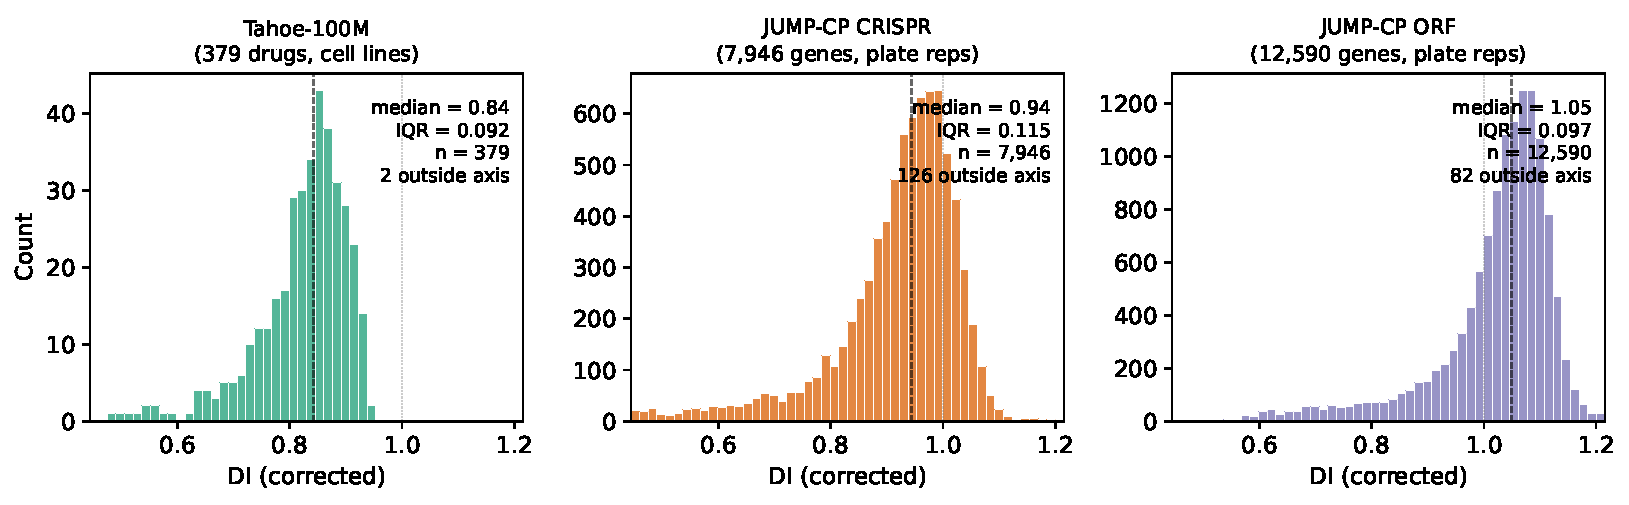
\includegraphics[width=\textwidth]{figures/fig_di_distributions.pdf}
\caption{Distribution of magnitude-corrected DI across the three new
atlas datasets.  Dashed lines mark medians; dotted lines mark
$\mathrm{DI} = 1$ (orthogonal signatures).  DI can exceed 1 when
signatures are anti-correlated across contexts.  All three panels share an
x-axis spanning the 0.5th--99.5th percentile of the pooled values; the count of
perturbations falling outside that window is stated in each panel.  Tahoe-100M
drug DI has the lowest median ($0.84$, against CRISPR $0.94$ and ORF $1.05$)
and the narrowest spread of the three on every measure: interquartile range
$0.092$ against $0.115$ and $0.097$, standard deviation $0.087$ against $0.131$
and $0.113$.  The narrower Tahoe distribution is expected from estimator
variance rather than from biology: DI is computed from $K$ contexts, and Tahoe
has a median $K$ of 49 against 5 for CRISPR and ORF.  CRISPR and ORF
distributions concentrate near 1 (near-orthogonal signatures across plate
replicates), reflecting the high baseline noise of morphological profiling at
plate-replicate resolution.}
\label{fig:distributions}
\end{figure}

\subsubsection*{Direction instability}

For a perturbation with $K \geq 5$ context-specific signatures
$\mathbf{s}_1, \ldots, \mathbf{s}_K \in \mathbb{R}^d$, direction
instability is
\begin{equation}
\mathrm{DI} = 1 - \frac{2}{K(K-1)} \sum_{i < j}
\frac{\mathbf{s}_i \cdot \mathbf{s}_j}
     {\|\mathbf{s}_i\| \, \|\mathbf{s}_j\|}.
\label{eq:di}
\end{equation}
DI $= 0$ when all signatures point in the same direction (perfectly
consistent perturbation), equals 1 when signatures are orthogonal,
and exceeds 1 when signatures are anti-correlated.  The excess is bounded:
$K$ unit vectors cannot be mutually anti-correlated, so
$0 \leq \mathrm{DI} \leq K/(K-1)$, giving a maximum of 2.000 at $K = 2$,
1.250 at $K = 5$, and 1.021 at $K = 49$.  For the Tahoe panel
($K = 49$) the maximum possible excess over 1 is therefore 0.021, and
``exceeds 1'' should be read quantitatively rather than as room for large
anti-correlation.  Note also that
$\mathrm{DI}_{\mathrm{corrected}}$ (Equation~\ref{eq:magnitude}) is a residual
plus an intercept and is not bounded by $K/(K-1)$; it is not interpretable as
$1 - \overline{\cos}$, and Figure~\ref{fig:distributions} plots the corrected
values.  By
construction, DI is a reparameterization of mean pairwise cosine
similarity (Pearson $r = -1.0$ between DI and $\overline{\cos}$).

\subsubsection*{Magnitude immunity and correction}

The first-order magnitude confound arises when a metric's expected value
changes with effect size: stronger perturbations mechanically produce
larger distances (or smaller ones, depending on the metric).  Cosine
similarity is ratio-scale---$\cos(\alpha \mathbf{s}_i,
\alpha \mathbf{s}_j) = \cos(\mathbf{s}_i, \mathbf{s}_j)$ for any
$\alpha > 0$---so DI is invariant to uniform rescaling of all
signatures.  This is the sense in which DI is ``immune by
construction'': the dominant confound pathway (stronger effect
$\to$ larger norm $\to$ larger distance) is algebraically cancelled.
The companion study \citep{tower2026confound} verified this empirically
across three modalities (LINCS, DepMap CRISPR, Perturb-seq), showing
that alternative metrics exhibit Cohen's $d = 0.55$--$2.65$ magnitude
confounding while DI shows none after correction.

A residual second-order correlation remains.  Weakly-acting
perturbations produce noisier signature estimates, and noise inflates
the average pairwise cosine dissimilarity even after unit-length
normalization.  We remove this residual confound by OLS regression of
raw DI on mean signature $L_2$ norm:
\begin{equation}
\mathrm{DI}_{\mathrm{corrected}} = \mathrm{DI}_{\mathrm{raw}}
  - \hat{f}(\overline{\|\mathbf{s}\|}) + \hat{\beta}_0,
\label{eq:magnitude}
\end{equation}
where $\hat{f}$ is the OLS prediction and $\hat{\beta}_0$ is the
intercept.  This correction is applied per dataset.
$\mathrm{DI}_{\mathrm{corrected}}$ is the primary metric throughout;
$\mathrm{DI}_{\mathrm{raw}}$ is reported for transparency.

\paragraph{What the correction leaves behind.}
$\hat{f}$ is a global linear fit on the untransformed norm, and the dependence
it removes is only the linear part of a monotonic, nonlinear relationship.  The
fit itself explains $R^2 = 0.081$ of raw DI in CRISPR
(Appendix~\ref{app:magnitude}), while a linear model of $\log$ mean norm and
magnitude~CV explains $R^2 = 0.478$ of the \emph{corrected} values in the same
dataset.  Magnitude-related structure therefore survives the correction in
CRISPR, and analyses on CRISPR DI control for norm and magnitude~CV explicitly
rather than relying on the correction alone (Section~\ref{sec:whatnot}).  The
residual is smaller in ORF ($R^2 = 0.313$) and small in Tahoe
($R^2 = 0.076$), consistent with Tahoe's higher signal-to-noise ratio.

\subsubsection*{Bootstrap confidence intervals}

For each perturbation, we resample the $K$ contexts with replacement
1{,}000 times and recompute DI on each bootstrap sample.  The 2.5th and
97.5th percentiles define the 95\% bootstrap confidence interval.  These
intervals quantify the stability of each DI estimate with respect to the
particular set of contexts observed.

\subsubsection*{Statistical framework}

All hypothesis tests use partial Spearman correlation with confound
control.  Spearman rather than Pearson correlation is used throughout because the
registered hypotheses are monotonic rather than linear, because DI and several
covariates (essentiality breadth, paralog count, cell-line count) are bounded or
heavily skewed, and because rank statistics limit the leverage of the extreme
di\_corrected values that the residual-plus-intercept definition admits.  The
partial correlation is computed by Pearson-residualizing
both variables against the covariate matrix (with intercept column),
then computing Spearman's $\rho$ on the residuals.  This method avoids
the bias of rank-then-residualize approaches, which produce spurious
partial correlations of $\rho \approx 0.05$--$0.25$ under the null at
large $n$ (verified in simulation; see pre-registration documents).
Confidence intervals use the Fisher $z$-transform with degrees of
freedom adjusted for the number of covariates.

Where the predictor is categorical rather than continuous, effect size is reported
as partial eta-squared from a one-way ANOVA,
\begin{equation}
\eta^2_p = \frac{SS_{\text{between}}}{SS_{\text{between}} + SS_{\text{within}}},
\end{equation}
which is the proportion of variance in the residualized outcome attributable to
class membership.  It replaces $\rho$ for the mechanism-of-action test because
mechanism-of-action class is unordered, so no monotonic relationship is defined
and a rank correlation would not be interpretable.  Degrees of freedom are reported with the
ANOVA, and significance is assessed by permutation of class labels rather than
against the $F$ reference distribution, since the class sizes are unequal and the
residualized outcome is not normal.

Every primary test applies two decision criteria simultaneously:
(i)~$p < \alpha$ (Bonferroni-corrected: $\alpha = 0.0125$ for Batch~1's
four primary tests, $\alpha = 0.0167$ for Batch~2A's three hypotheses
and Batch~3's three), and (ii)~the 95\% CI lower bound
exceeds $\pm 0.05$ in the predicted direction.  The CI floor is
necessary because at $n > 5{,}000$, effects as small as
$\rho = 0.03$ reach statistical significance.  Without the floor,
trivially small correlations would pass.

\subsubsection*{Data format}

The atlas is distributed as CSV files containing, for each perturbation:
$\mathrm{DI}_{\mathrm{raw}}$, $\mathrm{DI}_{\mathrm{corrected}}$,
bootstrap CI bounds, magnitude CV, mean signature norm, and number of
contexts.  Full data provenance and repository locations are listed in
the Data Availability section.


%% ====================================================================
\subsection*{Analysis plans and deviations}
\label{sec:integrity}
%% ====================================================================

All hypotheses, decision criteria, statistical methods, and analysis
code were frozen before execution.  Batch~1
(concordance, essentiality, knockout vs.\ overexpression, PRISM) was
frozen at commit SHA \texttt{0d07a01}; Batch~2A (expression variance,
drug selectivity, paralog count, paralog breadth) at commit SHA
\texttt{a17c125}; Batch~3 (MoA stratification, cross-cell-line CRISPR,
DepMap convergent) at commit SHA \texttt{4c34699}.  The pre-registration
documents specify the statistical method, Bonferroni correction levels,
decision criteria, power analyses, and interpretation guides for each
outcome.  All three documents are included in the repository.

The three plans were not written at the same time.  The first two were frozen
before any result in this study was known.  The third was written after the
results of the first two were known, and specifies three further hypotheses:
mechanism-of-action stratification, cross-cell-line replication of the
essentiality relationship, and a convergent test on dependency scores.  Its
hypotheses are prespecified with respect to their own outcomes and post hoc
with respect to the earlier results, and are marked as such wherever they are
reported.  Freeze times are verifiable against the repository history.

Two further disclosures attach to that third plan.  The mechanism-of-action
analysis is exploratory-then-confirmed: a raw, uncontrolled $\eta^2 \approx
0.42$ was seen during scoping before the plan was frozen, and the confirmatory
confound-controlled, permutation-tested version was unseen at freeze time.  For
the cross-cell-line replication, the analysis logic is byte-identical between
the frozen commit and the executed version; only the data download function was
changed after freezing, to correct S3 paths that returned 404 errors.  Both are
documented in the repository.

\subsubsection*{The confidence-interval floor}

At sample sizes above $n = 5{,}000$, trivially small effects reach
statistical significance.  The pre-registration introduced a uniform
CI lower-bound gate ($|$CI bound$| > 0.05$ in the predicted direction)
to prevent this.  The gate blocked expression variance
($\rho = 0.060$), which would have passed on $p$-value alone.
Paralog breadth ($\rho = -0.029$) fails on both criteria: its
$p = 0.017$ marginally exceeds the Bonferroni threshold and its CI
does not clear the floor.  In both cases, the effects explain less than
0.4\% of variance and lack biological plausibility as primary
explanations for DI variation.

\subsubsection*{Deviations}

Seven deviations from the pre-registration occurred during analysis.
All are data-wrangling corrections or sample-size discrepancies; none
alter the statistical method, decision criteria, or interpretation
framework.

\paragraph{DepMap version.}
All DepMap analyses use the pre-registered 24Q4 release (figshare
article 27993248): Chronos dependency scores (file 51064667; 1{,}178
cell lines, 17{,}916 genes) for the essentiality test, expression
(file 51065489; 1{,}673 cell lines, 19{,}193 genes) for expression
variance and paralog tests.
Initial runs inadvertently used 22Q2 Chronos (essentiality) and 24Q2
expression (expression variance, paralogs).  Re-running on the correct 24Q4 release changed no
verdicts: the essentiality test moved from $\rho = -0.330$ to $-0.332$,
expression variance from $0.064$ to $0.060$, and paralog count/breadth
were identical to three decimal places.

\paragraph{Same-modality concordance matching method.}
The pre-registration specified InChIKey matching for drug concordance.
An initial run erroneously used case-insensitive drug-name matching
($n = 114$, $\rho = -0.003$), which introduced approximately 38
spurious pairs from salt forms, stereoisomers, and name collisions.
Reverting to InChIKey matching via PubChem CID cross-reference
($n = 76$, $\rho = 0.254$) moved toward the pre-registered method,
resolving the spurious null.  The InChIKey result is the pre-registered analysis; the
name-matched result is documented in Appendix~\ref{app:a1matching}.

\paragraph{Batches 1--2A deviations.}
(i)~Cross-modal concordance yielded $n = 378$ instead of the estimated $n = 330$, because
\texttt{pert\_iname} matching recovered more valid InChIKey pairs than
anticipated.
(ii)~\texttt{pert\_iname} was used instead of \texttt{pert\_id} for
LINCS metadata lookup; \texttt{pert\_id} matching was a data-wrangling
error yielding only 8 compounds.
(iii)~Context definitions differ across datasets (cell lines vs.\ plate
replicates); see Section~\ref{sec:atlas} and Section~\ref{sec:discussion}.
(iv)~Drug selectivity yielded $n = 75$ instead of the estimated $n \sim 1{,}000$ due
to the small LINCS-PRISM overlap after viability filtering.
(v)~Nine genes were dropped from the paralog tests due to missing
expression values, leaving $n = 6{,}894$ (paralog count) and
$n = 6{,}882$ (paralog breadth).
(vi)~The CRISPR and ORF panels contain 7{,}946 and 12{,}590 perturbations
against the plan's pre-analysis estimates of 7{,}948 and 15{,}121; both
differences follow deterministically from the quality filter and neither
affects a decision criterion.

\paragraph{Batch 3 deviations.}
(i)~Experiment~F: The scoping disclosure (raw $\eta^2$ observed before
freeze) is described above.  The confirmatory analysis
(confound-controlled, permutation-tested) was unseen at freeze time.
(ii)~Experiment~G: The pre-registration estimated $n \approx 160$ shared
genes; the actual overlap with DepMap is $n = 128$ (deterministic:
genes present in both cell lines with non-zero signature norms).
The data download function was modified post-freeze to use the correct
S3 paths; the analysis logic (DI computation, correlation, CI) is
byte-identical to the frozen version.
(iii)~After obtaining the Experiment~G result, bootstrap and
timepoint-stratified sensitivity analyses were run exploratorily.
These were not pre-registered and are excluded from the manuscript
(documented in \texttt{DEVIATIONS.md}).


%% ====================================================================
\section{Results}\label{sec:results}
\subsection{Concordance across measurement modalities}
\label{sec:concordance}
%% ====================================================================

The atlas is useful only if DI reflects a biological property of
perturbations rather than a measurement artifact of any single platform.
Two pre-registered concordance tests assess this by comparing
DI values for the same compounds measured in different datasets.  An
exploratory check against PRISM cell viability, a scalar outcome with a
different noise structure, is reported in Appendix~\ref{app:prism}.

\subsubsection{Transcriptomic against morphological}

Compounds present in both LINCS L1000 (transcriptomic DI) and JUMP-CP
Cell Painting (morphological DI) were matched by InChIKey connectivity
prefix (14 characters).  Of the matched set, $n = 378$ compounds have
$\geq 5$ contexts in both datasets.

Partial Spearman $\rho = 0.190$ (95\% CI $[0.090, 0.285]$,
$p = 2.1 \times 10^{-4}$), controlling for LINCS $n_{\mathrm{contexts}}$
as one covariate.  The CI lower bound (0.090) exceeds the 0.05 floor,
and $p < 0.0125$.  This test passes both pre-registered criteria.

The effect size falls in the ``weakly concordant'' bin
($0.15 \leq \rho < 0.30$) defined in the pre-registration, consistent
with the expectation that cross-modal comparisons capture only the
fraction of biology shared between gene expression and cell morphology
\citep{haghighi2022crossmodal}.  The concordance is weak but genuine:
compounds whose transcriptomic signatures vary across cell lines also
produce variable morphological profiles, and this relationship survives
confound control.

\subsubsection{Transcriptomic against transcriptomic}

Drugs present in both LINCS L1000 and Tahoe-100M were matched by
InChIKey connectivity prefix, verified via PubChem CID cross-reference.
This yielded $n = 76$ overlapping compounds (fewer than the
pre-registered estimate of $n \approx 103$, because some Tahoe drugs
lack PubChem CID annotations mapping to LINCS InChIKeys).  LINCS DI is
computed in $\mathbb{R}^{978}$ (landmark genes) while Tahoe DI is
computed in $\mathbb{R}^{\sim 62{,}000}$ (full transcriptome).  Because
cosine similarity is invariant to positive rescaling, DI values are
comparable across feature spaces of different dimensionality.

Partial Spearman $\rho = 0.254$ (95\% CI $[0.027, 0.456]$,
$p = 0.029$), controlling for LINCS and Tahoe $n_{\mathrm{contexts}}$
(two covariates).  This test \textbf{fails}: the CI lower bound
(0.027) does not clear the 0.05 floor, and $p = 0.029$ exceeds the
Bonferroni threshold ($\alpha = 0.0125$).

The failure is one of statistical power, not absence of concordance.
The point estimate ($\rho = 0.254$) is larger than the cross-modal result
($\rho = 0.190$), and the pre-registered power analysis predicted this
outcome: at $n = 76$, the study achieves 80\% power only for true
effects $\geq 0.35$.  We interpret this pattern as a sample-size
artifact---the LINCS-Tahoe overlap ($n = 76$) is far smaller than
LINCS-JUMP ($n = 378$)---rather than evidence that DI transfers better
across modalities than within one.  A deviation in the matching method
is disclosed in Section~\ref{sec:integrity}.

\subsection{Mechanism-of-action structure}
\label{sec:moa}
%% ====================================================================

\paragraph{Scoping disclosure.}
A raw, uncontrolled one-way ANOVA of DI on mechanism-of-action class was computed
during scoping and gave $\eta^2 \approx 0.42$; that number was seen before the
analysis plan was frozen.  The confirmatory test specified in the plan is the
confound-controlled, permutation-tested version reported below, whose result was
unseen at freeze time.  This analysis is therefore exploratory-then-confirmed.

Batches~1 and~2A established which gene-level properties fail to explain DI.
The natural follow-up is whether DI varies systematically with drug
mechanism-of-action class.  If core-machinery inhibitors (targeting
fundamental cellular processes) show low DI while receptor-signaling
drugs (engaging cell-type-specific pathways) show high DI, then DI
captures biologically interpretable structure, and the atlas stratifies
drug classes in a useful way.

Because DI depends mechanically on profiling depth (number of cell
lines) and MoA classes may differ in profiling depth, the primary
analysis uses residualized DI: raw DI residualized on
$n_{\mathrm{cell\,lines}}$ and mean signature norm via OLS.  One-way
ANOVA of residualized DI on MoA class (80 classes with $\geq 5$ drugs,
1{,}031 drugs total; $\mathrm{df} = 79, 951$) yields partial
$\eta^2 = 0.201$.  The raw
(uncontrolled) $\eta^2$ is 0.417; controlling for profiling depth and
signal strength halves the effect, confirming that the confound control
is load-bearing.

A 1{,}000-permutation null (shuffling MoA labels, preserving class
sizes) produced a null distribution with mean $= 0.077$,
SD $= 0.012$, 99th percentile $= 0.111$.  The observed
$\eta^2 = 0.201$ exceeds the 99th percentile and the empirical
permutation $p < 0.001$.  Both pre-registered criteria are met.

The biological pattern is interpretable.  The lowest-DI MoA classes are
mTOR inhibitors, HDAC inhibitors, HSP inhibitors, and PI3K
inhibitors---drugs targeting core cellular machinery
\citep{santos2017drug} that operates uniformly across cell types.  The highest-DI classes are serotonin
receptor agonists, histamine receptor agonists, GABA receptor
antagonists, and PPAR receptor agonists---drugs acting through
receptor-mediated signaling pathways whose expression and coupling vary
across cell lineages.

Mechanism-of-action class therefore accounts for a fifth of
residualized DI variance, and the classes separate along a pharmacologically
interpretable axis rather than an arbitrary one.



%% ====================================================================
\subsection{Gene-level properties that do not explain DI}
\label{sec:whatnot}
%% ====================================================================

Five pre-registered experiments (Batches~1 and 2A) tested whether DI
variation across genes and drugs can be explained by simpler biological
properties.  All five fail their pre-registered criteria, and each
failure constrains the interpretation of DI in a specific way.
Figure~\ref{fig:forest} shows each effect against the $\pm 0.05$ confidence-interval
floor, which is what separates the failures from the two passes.
Table~\ref{tab:results} summarizes the full scorecard including the
replication and divergence tests (Section~\ref{sec:batch3}).

\vspace{1em}
\begin{table}[htbp]
\centering
\caption{Pre-registered experiment results.  Batches~1--2A use partial
Spearman $\rho$ with confound control ($\alpha = 0.0125$ for Batch~1,
$0.0167$ for Batch~2A) except the KO vs.\ OE test (raw Spearman +
permutation null).  Batch~3 ($\alpha = 0.0167$, three tests) was
prompted by peer review; Experiment~F reports partial $\eta^2$ instead
of $\rho$.  ``CI gate'' indicates that the 95\% CI lower bound did not
clear the $\pm 0.05$ threshold in the predicted direction.
$^{\ddagger}$Reported in Appendix~\ref{app:prism}: uncorrected $p$, no covariate
adjustment, $n = 75$.}
\label{tab:results}
\small
\begin{tabular}{@{}llrrrl@{}}
\toprule
\textbf{Batch} & \textbf{Hypothesis} & $n$ &
\textbf{Effect} & $p$ & \textbf{Verdict} \\
\midrule
1 & Cross-modal concordance & 378 & $\rho = 0.190$ & $2.1 \times 10^{-4}$ & \textbf{PASS} \\
1 & Same-modality concordance & 76 & $\rho = 0.254$ & 0.029 & FAIL (CI gate) \\
1 & Essentiality $\to$ high DI & 7{,}653 & $\rho = -0.332$ & ${\sim}0$ & FAIL (wrong sign) \\
1 & KO $\approx$ OE DI & 5{,}220 & $\rho = 0.011$ & 0.43 & FAIL (null) \\
2A & Expression variance & 7{,}802 & $\rho = 0.060$ & $1.1 \times 10^{-7}$ & FAIL (CI gate) \\
2A & Drug selectivity & 75 & $\rho = 0.144$ & 0.22 & FAIL (underpowered) \\
2A & Paralog count & 6{,}894 & $\rho = -0.007$ & 0.57 & FAIL (null) \\
2A & Paralog breadth & 6{,}882 & $\rho = -0.029$ & 0.017 & FAIL (CI gate $+ \, p$) \\
\midrule
3 & MoA stratification (F) & 1{,}031 & $\eta^2 = 0.201$ & ${<}0.001$ & \textbf{PASS} \\
3 & Cross-cell-line ess.\ (G) & 128 & $\rho = -0.264$ & 0.003 & Directional (exploratory) \\
3 & DepMap convergent (H) & 17{,}916 & $\rho = +0.811$ & ${\sim}0$ & FAIL (wrong sign) \\
\midrule
\multicolumn{6}{@{}l}{\textit{Exploratory}} \\
1 & Viability concordance$^{\ddagger}$ & 75 & $\rho = 0.359$ & 0.0016 & Exploratory \\
\bottomrule
\end{tabular}
\end{table}

\begin{figure}[t]
\centering
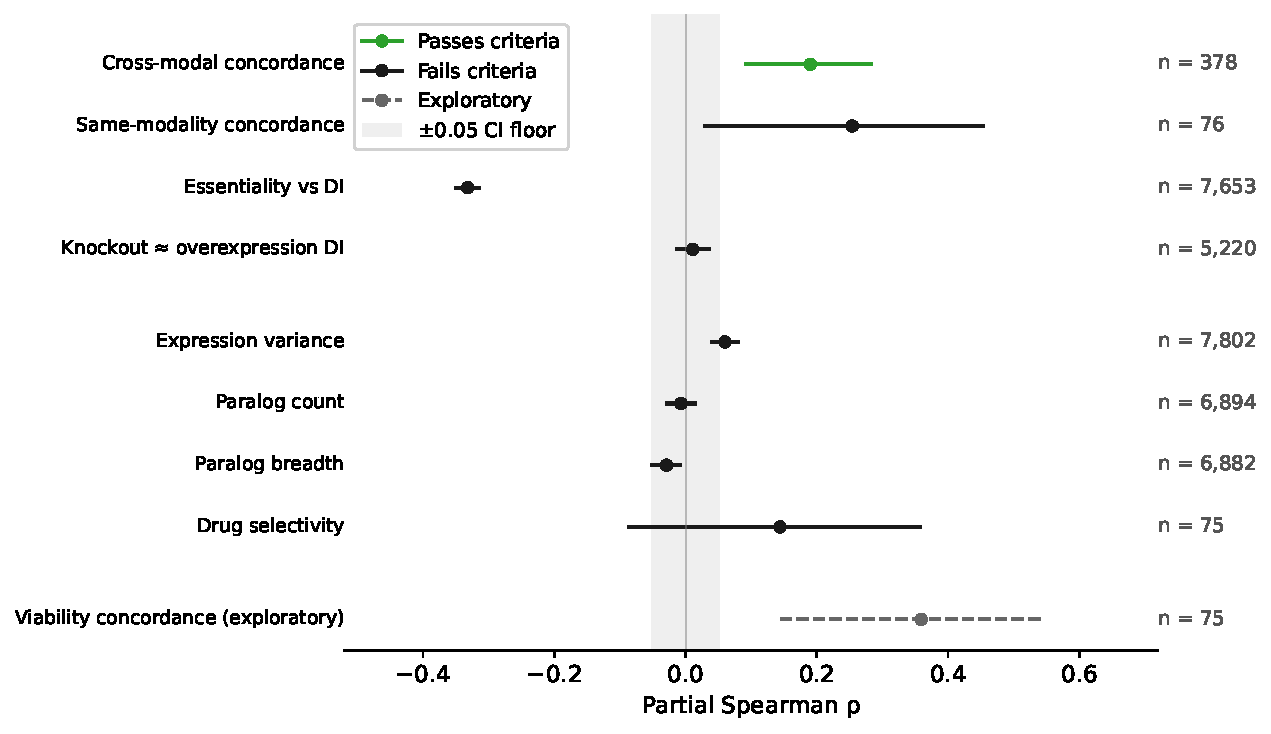
\includegraphics[width=0.85\textwidth]{figures/fig_forest_plot.pdf}
\caption{Pre-registered experiment results (Batches~1--2A).  Each point
shows the partial Spearman $\rho$ (or raw Spearman for the knockout vs.\
overexpression test) with 95\% confidence intervals.  The gray band
marks the $\pm 0.05$ CI floor: a test passes only if its CI lower bound
clears this band in the predicted direction.  Same-modality concordance
has a larger point estimate ($\rho = 0.25$) than cross-modal ($\rho =
0.19$) but fails because its CI lower bound ($0.027$) falls inside the
floor at $n = 76$.  Only cross-modal concordance passes both
pre-registered criteria; the seven primary failures delimit what DI
measures.  The mechanism-of-action, replication and divergence results are
reported in Sections~\ref{sec:moa} and~\ref{sec:batch3} and
Table~\ref{tab:results}.}
\label{fig:forest}
\end{figure}


\subsubsection{Essentiality breadth}

The pre-registration predicted that broadly essential genes would show
high morphological DI: genes required in many cell types should produce
context-dependent phenotypic disruption.  The observed correlation is
large, precisely estimated, and in the opposite direction.  Partial
Spearman $\rho = -0.332$ (95\% CI $[-0.352, -0.312]$, $p \approx 0$,
$n = 7{,}653$), controlling for $n_{\mathrm{contexts}}$.  Essentiality
breadth (fraction of DepMap 24Q4 cell lines with Chronos score
$< -0.5$; \citealp{tsherniak2017depmap, dempster2021chronos,
funk2022phenotypic}) predicts \emph{lower} DI,
accounting for approximately 11\% of variance.

\paragraph{Attenuation under signal-strength control.}
Because CRISPR DI is computed across plate replicates, a purely measurement-side
pathway predicts the same sign: an essential gene produces a large phenotype,
a large phenotype gives a higher signal-to-noise ratio, replicate signatures
then agree more closely, and DI falls.  That pathway requires no appeal to
functional constraint.  It is present in these data: essentiality breadth
correlates with mean signature norm at Spearman $\rho = +0.259$, and corrected
DI retains structure related to signal strength ($\rho = -0.212$ with mean
norm, $\rho = +0.279$ with magnitude~CV).

Adding mean norm to the covariate set moves the partial correlation from
$-0.332$ to $-0.243$; adding magnitude~CV as well moves it to
$\rho = -0.189$ (95\% CI $[-0.211, -0.168]$, $p \approx 0$, $n = 7{,}653$), a
reduction of roughly 43\%.  \textbf{We report $\rho = -0.189$ as the effect
after signal-strength control, and treat it rather than $-0.332$ as the
quantity the functional-constraint reading has to explain.}  Roughly half of
the raw association is attributable to signal strength in a metric that is
magnitude-invariant by construction, which is itself a constraint on how far
that construction protects against magnitude.

Mean norm may be a mediator rather than a confounder here, since knocking out
an essential gene should produce a large phenotype.  The design cannot separate
the two, and that ambiguity is the reason the residual association is reported
as a bound rather than as an estimate of functional constraint.

Figure~\ref{fig:essentiality} shows the relationship.
The sign-flip admits a natural interpretation, which we emphasize
is \emph{post-hoc}: the pre-registration confused two senses of
context-dependence.  Essential genes affect many cell types, but they
affect them in the same way.  A gene required for mitosis, ribosome
assembly, or DNA repair produces a stereotyped catastrophe regardless of
cellular identity.  Functional constraint makes the downstream
phenotypic consequences uniform across contexts, yielding low DI.  Genes
with high DI tend to be selectively essential or non-essential---their
knockout phenotypes interact with cell-type-specific pathways,
producing variable consequences across the panel.

This interpretation generates a falsifiable prediction: among
non-essential genes, those with tissue-restricted expression (active in
few cell types) should show \emph{higher} DI than ubiquitously expressed
non-essential genes, because tissue-restricted function implies
cell-type-specific downstream consequences.  We flag this as a candidate
for prospective pre-registration.

The result is consistent with the phenotypic landscape of essential genes being
structured by functional constraint \citep{hart2015crispr, meyers2017crispr}.
The two morphological atlases cited here do not test cross-cell-type uniformity
of phenotypic \emph{direction}: \citet{funk2022phenotypic} is an optical pooled
screen in a single HeLa line, and \citet{ramezani2025periscope} maps morphology
across A549 and HeLa without comparing the direction of a gene's phenotype
between them.  Neither supports a claim about uniform direction across cell
types, and none is made here.  DepMap pan-essentiality is likewise uniformity
of a scalar viability measure, not of direction in a multivariate phenotype;
Experiment~H (Section~\ref{sec:batch3}) shows what happens when the two are
conflated.

\begin{figure}[t]
\centering
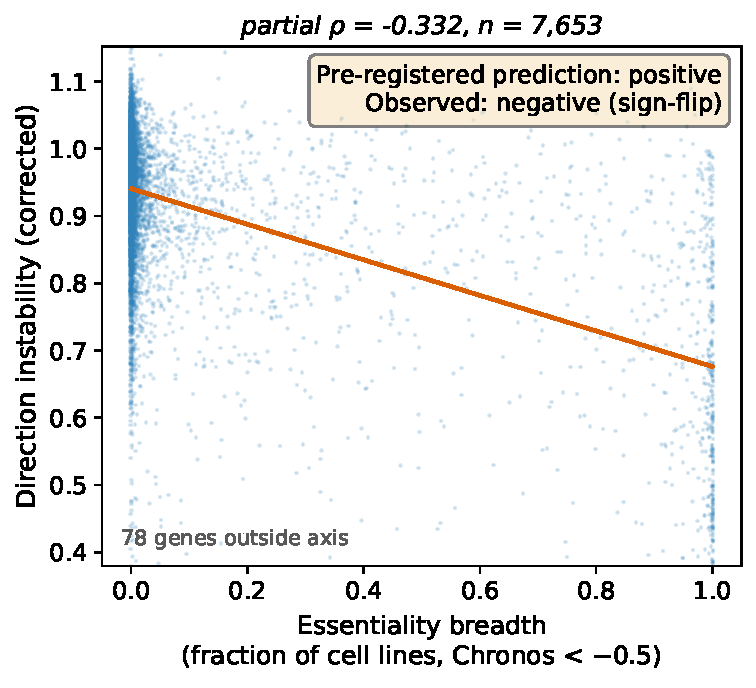
\includegraphics[width=0.65\textwidth]{figures/fig_essentiality_scatter.pdf}
\caption{Essentiality breadth (fraction of DepMap cell lines with
Chronos $< -0.5$) vs.\ magnitude-corrected DI for $n = 7{,}653$ JUMP-CP
CRISPR genes.  The pre-registration predicted
a positive correlation; the observed relationship is negative (partial
$\rho = -0.332$ controlling for $n_{\mathrm{contexts}}$).  Genes
essential across many cell lines show low DI, and selectively essential or
non-essential genes show higher DI.  A post-hoc reading is that functional
constraint makes downstream phenotypic consequences uniform across contexts; the
association attenuates to $\rho = -0.189$ once signal strength is controlled.
Line: OLS fit.}
\label{fig:essentiality}
\end{figure}


\subsubsection{Knockout against overexpression}

If context-dependence were an intrinsic property of genes, then a
gene's knockout DI and its overexpression DI should correlate.
Spearman $\rho = 0.011$ (95\% CI $[-0.016, 0.038]$, $p = 0.43$,
$n = 5{,}220$ genes with $\geq 5$ replicates in both CRISPR and ORF).
A mandatory permutation null (1{,}000 label shuffles preserving plate
structure; Appendix~\ref{app:permutation}) yielded a null distribution
with mean $= 0.0003$, SD $= 0.014$, 95th percentile $= 0.023$.  The
observed $\rho = 0.011$ falls within the null (permutation
$p = 0.215$).

At $n = 5{,}220$, the study had power to detect effects as small as
$\rho = 0.04$ (SE $\approx 0.014$).  The null is well-powered: losing a
protein and gaining excess protein engage different molecular
mechanisms---loss-of-function versus gain-of-function---and those
mechanisms interact with cellular context independently
\citep{badonyi2025lof, chandrasekaran2024cpjump1}.

Figure~\ref{fig:ko_vs_oe} shows the absence of any relationship.
This result constrains the theoretical scope of DI.  A gene is
context-dependent in a particular way (knockout, overexpression,
pharmacological inhibition), and DI values from one perturbation type
carry no information about another.  A DI atlas must be stratified by
perturbation mechanism.

\begin{figure}[t]
\centering
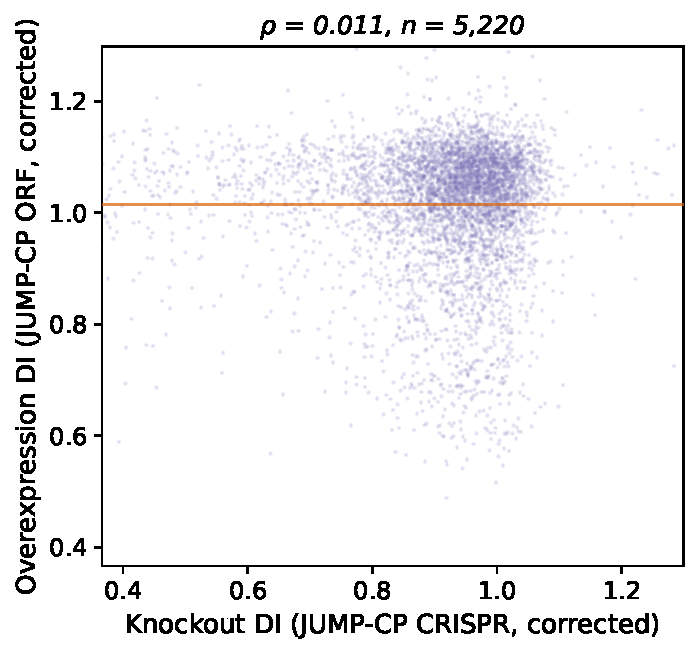
\includegraphics[width=0.65\textwidth]{figures/fig_ko_vs_oe_scatter.pdf}
\caption{Knockout DI (JUMP-CP CRISPR) vs.\ overexpression DI (JUMP-CP
ORF) for $n = 5{,}220$ genes profiled under both perturbation types.
Spearman $\rho = 0.011$ ($p = 0.43$): no relationship.  A gene's
knockout DI does not predict its overexpression DI, so DI does not behave as a
stable property of the target gene.  Line: OLS fit, slope indistinguishable from
zero.}
\label{fig:ko_vs_oe}
\end{figure}


\subsubsection{Expression variance, paralog count, paralog breadth}

Three plausible proxies for context-dependence---expression variance
across cell lines, paralog count, and paralog expression breadth---were
specified in the second analysis plan.  All three fail after confound control, and the
failures are informative about the structure of the confounds.

\paragraph{Expression variance.}
Partial Spearman $\rho = 0.060$ (95\% CI $[0.038, 0.082]$,
$p = 1.1 \times 10^{-7}$, $n = 7{,}802$), controlling for
$n_{\mathrm{contexts}}$.  The correlation is statistically unambiguous
but biologically negligible: $\rho = 0.060$ explains less than 0.4\% of
variance.  The CI lower bound (0.038) does not clear the 0.05 floor.
Expression variance captures a real but negligible relationship: genes
with variable expression produce marginally more variable knockout
phenotypes.  The remaining DI variation reflects factors beyond
expression variance.  Expression data from DepMap 24Q4
(OmicsExpressionProteinCodingGenesTPMLogp1.csv, 1{,}673 cell lines,
19{,}193 genes).

\paragraph{Paralog count.}
Partial Spearman $\rho = -0.007$ (95\% CI $[-0.031, 0.017]$,
$p = 0.57$, $n = 6{,}894$), controlling for $n_{\mathrm{contexts}}$ and
mean expression level.  The raw Spearman correlation was
$\rho = 0.038$ ($p = 0.002$)---a statistically significant positive
association.  The partial correlation is zero.  The raw association
existed because highly expressed genes have more paralogs (gene family
expansion correlates with expression level) and independently have
higher DI.  Controlling for expression removes the confound entirely.
The significant raw association ($p = 0.002$) evaporates under
covariate control.
Paralog data from Ensembl BioMart (GRCh38, Ensembl~113).

\paragraph{Paralog expression breadth.}
Among genes with $\geq 1$ expressed paralog ($n = 6{,}882$), partial
Spearman $\rho = -0.029$ (95\% CI $[-0.053, -0.005]$, $p = 0.017$),
controlling for $n_{\mathrm{contexts}}$ and mean expression level.  The
sign is correct (broader paralog compensation predicts lower DI, as
hypothesized), but $p = 0.017$ exceeds the Bonferroni threshold
($\alpha = 0.0167$) and the CI upper bound ($-0.005$) does not
clear $-0.05$.  Both criteria fail: neither $p$-value nor CI gate passes.
The raw correlation
($\rho = -0.117$, $p \sim 10^{-22}$) is substantially larger,
indicating that expression-level confounds inflate the apparent
paralog-breadth effect as well.


\subsubsection{Drug selectivity}

Partial Spearman $\rho = 0.144$ (95\% CI $[-0.088, 0.360]$,
$p = 0.22$, $n = 75$), controlling for LINCS $n_{\mathrm{contexts}}$.
The primary metric is magnitude-corrected Gini of PRISM kill depth,
residualizing raw Gini against mean kill magnitude to remove the
mechanical confound between potency and selectivity.  The correction
reduced the apparent association from $\rho = 0.275$ (raw Gini) to
$\rho = 0.144$ (corrected Gini), confirming the magnitude confound is
real.

The CI spans $[-0.088, 0.360]$, consistent with anything from no effect
to a moderate one.  The pre-registration assumed $n \sim 1{,}000$;
actual overlap between LINCS drugs and PRISM compounds with
$|\mathrm{mean\;LFC}| \geq 0.01$ is $n = 75$, an order of magnitude
smaller.  This experiment cannot distinguish a real $\rho = 0.15$ effect
from zero.


%% ====================================================================
\subsection{Replication and construct divergence}
\label{sec:batch3}
%% ====================================================================

\subsubsection{Essentiality across two cell lines}

The essentiality sign-flip reported above ($\rho = -0.33$, $n = 7{,}653$) was
computed on plate-replicate DI within a single cell line (U2OS).  Plate
replicates measure technical reproducibility, and reviewers asked whether
the sign-flip reflects biology or plate-level noise.

The cpg0000 pilot dataset (Cell Painting Gallery) provides CRISPR
profiles from two cell lines: A549 (10 plates) and U2OS (8 plates).
With $K = 2$ cell lines, DI degenerates to a single pairwise cosine
distance: $\mathrm{DI} = 1 - \cos(\mathbf{s}_{\mathrm{A549}},
\mathbf{s}_{\mathrm{U2OS}})$.  This is geometrically valid but
extremely noisy per gene (no averaging over pairs).  Cell line
assignments were obtained from the companion metadata repository
\citep{chandrasekaran2024cpjump1}.

Of 128 genes with profiles in both cell lines, Spearman
$\rho = -0.264$ (95\% CI $[-0.418, -0.095]$, $p = 0.003$,
$n = 128$).  The correlation is negative, statistically significant
at $\alpha = 0.0167$, and the CI excludes zero.  The pre-registered
verdict is \textbf{directional replication}: the essentiality sign-flip
observed on plate replicates holds in direction on true
cross-cell-line data, giving provisional directional evidence against a
purely technical reading
to biological context-dependence.

The point estimate ($\rho = -0.26$) is smaller than the plate-replicate result
($\rho = -0.33$), consistent with the expected attenuation from $K = 2$
noise.  The CI is wide ($[-0.42, -0.10]$), reflecting the small
sample size ($n = 128$ against $7{,}653$) and the
degeneracy of single-cosine DI.  This experiment narrows the
interpretation of the sign-flip; it does not close it.  Properly powered
cross-cell-line replication requires datasets with $K \geq 5$ cell
lines per gene, such as future expansions of JUMP or single-cell CRISPR
screens \citep{tahoe2025}.

\subsubsection{Scalar dependency variability}

The biological interpretation of the essentiality sign-flip---functional
constraint suppresses context-dependent phenotypes---predicts that the
same pattern should appear in dependency scores: broadly essential genes
should show uniform dependency across cell lines (low variability),
while selectively essential genes should show variable dependency (high
variability).  Testing this on DepMap Chronos scores provides convergent
evidence from a fundamentally different measurement.

Partial Spearman $\rho = +0.811$ (95\% CI $[0.806, 0.816]$,
$p \approx 0$, $n = 17{,}916$), controlling for the number of
non-missing Chronos values per gene.  The pre-registered prediction
was negative ($\rho < -0.05$); the observed correlation is strongly
positive.  This test fails.

We hypothesize the failure reflects a construct divergence rather than
a biological contradiction.  DepMap essentiality breadth
(fraction of cell lines with Chronos $< -0.5$) and dependency-score SD
are different geometric constructs from morphological DI.  Morphological
DI measures pairwise cosine distance between high-dimensional vectors;
dependency-score SD measures the spread of scalar values.  A gene
essential in many cell lines has a wider range of Chronos
scores (some near $-1$, others near $-0.5$), producing high SD.  The
positive correlation may reflect this scalar-range property: broadly
essential genes show high dependency-score variability because
the Chronos scale admits more spread as more cell lines cross the
essentiality threshold.  Consistent with this interpretation,
dependency-score SD correlates with Chronos score range at
$\rho = 0.83$: SD is largely a proxy for the mechanical range of
scores a gene spans, which widens as more cell lines cross the
essentiality threshold ($\rho = 0.79$ between score range and
breadth).

The failure exposes a construct divergence: the
functional-constraint hypothesis makes different predictions depending
on whether context-dependence is measured as vector cosine distance
(morphological DI) or scalar variability (dependency-score SD).  The
morphological sign-flip stands; the convergent pathway through DepMap SD
does not replicate it.  A convergent test using a vector-valued DepMap
representation (such as gene-expression signatures of knockout effects
across cell lines) would avoid this scalar artifact.


%% ====================================================================
\section{Discussion}
\label{sec:discussion}
%% ====================================================================

\subsection{What DI measures---and what it does not}

Eleven pre-registered experiments produce a consistent characterization
of direction instability.  DI carries a modest cross-modal
component, evidence that it is not specific to one measurement platform.
It is perturbation-type-specific: knockout and overexpression of the same
gene produce unrelated DI profiles, so DI does not behave as a stable
property of the target gene.  Broad essentiality is associated with lower
DI after measured signal-strength adjustment; functional constraint
producing stereotyped disruption is one hypothesis that would account for
this, and the association directionally replicates on true cross-cell-line
CRISPR data ($\rho = -0.26$, cpg0000 pilot).  Three
plausible proxy explanations---expression variance, paralog count,
paralog breadth---each explain less than 0.4\% of DI variance after
confound control.

DI is also mechanism-structured at the pharmacological level: drug MoA
classes explain 20\% of residualized DI variance, with an interpretable
pattern distinguishing core-machinery inhibitors (low DI) from
receptor-signaling drugs (high DI).  Cross-context consistency is
complementary to selectivity: a highly selective drug can still show high DI if
its target pathway is wired differently across cell types.

The DepMap convergent test exposes a boundary of the
functional-constraint interpretation.  Dependency-score SD and
essentiality breadth correlate positively ($\rho = +0.81$), opposite to
the morphological sign-flip, because the scalar SD estimand mechanically
inflates with the Chronos score range.  The functional-constraint
hypothesis makes different predictions depending on whether
context-dependence is measured as vector cosine distance or scalar
variability.  The morphological sign-flip is about directional
consistency of high-dimensional profiles; DepMap SD indexes scalar
spread.  Future convergent tests should use vector-valued representations
of dependency effects.

This combination of positive, negative, and failed results shows that DI
captures how perturbation mechanisms interact with
cell-type-specific biology.  It is not reducible to essentiality breadth,
expression variance, or paralog structure, though the association with
essentiality breadth survives adjustment at $\rho = -0.189$.  Other untested features
such as protein interaction network topology or chromatin accessibility
might correlate with DI; the present results constrain the space of
explanations without exhausting it.  For atlas users, the practical
implication is that DI provides information beyond what is available
from essentiality screens, expression atlases, or paralog databases.

\subsection{The resource}

The atlas provides magnitude-corrected DI values with bootstrap
confidence intervals for 8{,}949 LINCS drugs, 379 Tahoe drugs, 7{,}946
CRISPR knockouts, and 12{,}590 ORF overexpressions.  The companion JUMP-CP
compound DI values (25{,}254 compounds) are available from a prior
study \citep{tower2026confound}.  Together, these cover the
perturbation-biology datasets most widely used for drug mechanism
prediction, gene function annotation, and virtual screening
benchmarks.

The atlas is designed for downstream integration.  Each row provides the
columns needed for a secondary analysis: corrected DI, raw DI, CI
bounds, mean signature norm, magnitude CV, and number of contexts.
Pre-registration documents, analysis scripts, and result JSON files are
released alongside the data.

\subsection{Limitations}

\paragraph{Statistical power.}
The PRISM viability analysis ($\rho = 0.359$, $n = 75$) is exploratory:
uncorrected $p$-value, no covariate adjustment, small sample.  It
provides corroboration only.
The same-modality concordance test (LINCS-Tahoe, $n = 76$) was
underpowered by design: the LINCS-Tahoe compound overlap is
structurally small.  The point estimate ($\rho = 0.254$) is consistent
with genuine concordance, but the wide CI ($[0.027, 0.456]$) precludes a
firm conclusion.
The drug selectivity test is underpowered at $n = 75$ and cannot
distinguish a moderate effect from zero.  Both underpowered tests are
data-limited: the small $n$ reflects the structural size of the dataset
intersection, not a design choice.  We report them for completeness and
for the atlas resource record, not as adjudicated hypotheses.
Experiment~G computes DI from $K = 2$ cell lines, the minimum for a
pairwise comparison.  With $K = 2$, DI is a single cosine distance
rather than an average over pairs, making it extremely noisy per gene.
No magnitude correction was applied ($n = 128$ is too small for
meaningful OLS), and no bootstrap CIs are possible.  The A549 plates
vary in timepoint (96h vs.\ 144h) and antibiotic treatment, introducing
uncontrolled confounds.  The experiment's value is as a directional
check, not a definitive test.

\paragraph{Construct and interpretation.}
Context definitions vary across datasets.  LINCS and Tahoe use cell
lines as contexts; JUMP-CP CRISPR and ORF use plate replicates.  Plate
replicates sample technical variability within one cell line, while cell
lines sample biological variability across cell types.  DI computed over
plate replicates measures reproducibility within a fixed biological
context, whereas DI over cell lines measures context-dependence across
biological contexts.  Cross-dataset comparisons match on context type,
but the CRISPR/ORF DI values used in the essentiality,
mechanism-specificity, and proxy tests index technical variability rather
than biological context-dependence.  Extending the atlas to single-cell
CRISPR screens with cell-line diversity \citep{tahoe2025} would resolve
this asymmetry.
The essentiality sign-flip interpretation (functional constraint
suppresses DI) is post-hoc.  The pre-registration predicted the
opposite sign.  The mechanistic explanation is plausible and connects to results in
functional genomics \citep{funk2022phenotypic, ramezani2025periscope}, but it
was generated after observing the data.  A companion preprint by the same
author reports that universal-essential knockdowns diverge rather than converge
across cell types in Perturb-seq data ($d = 0.60$,
$p_{\mathrm{perm}} < 10^{-4}$; \citealp{tower2026validity}); that finding is
not independent of the present work, and its direction is opposite to the
uniform-disruption reading, so it is recorded here as an open tension rather
than as support.  \citet{replogle2022perturbseq} bear directly on the question:
genome-scale Perturb-seq in K562 and RPE1 finds only partial concordance of
knockdown phenotypes across the two lines, which is consistent with
context-dependence being widespread and argues against reading low DI as
evidence of uniform cross-cell-type disruption.  Prospective testing of a
falsifiable prediction---among non-essential genes, tissue-restricted
expression should positively predict DI
(Section~\ref{sec:whatnot})---would convert this post-hoc
rationalization into a validated mechanism.
Experiment~F is exploratory-then-confirmed (scoping disclosure,
Section~\ref{sec:batch3}); the confound-controlled $\eta^2 = 0.20$ is
the primary result.

Experiment~H exposes a construct divergence: scalar dependency-score SD
and vector cosine DI measure different geometric properties of
context-dependence.  The positive $\rho = +0.81$ does not falsify the
morphological sign-flip; it shows that the functional-constraint
hypothesis generates different predictions under different operationalizations.

\paragraph{Data scope.}
LINCS L1000 has well-documented batch effects across production sites
and plates \citep{subramanian2017next}.  If a drug was profiled across
batches, batch-driven direction differences would inflate DI
independently of biology.  The companion study's split-half stability
analysis provides indirect reassurance, but a direct test of whether DI
correlates with batch structure has not been performed.
All DI values are computed at the dose used in each screening campaign.
Dose-response effects could change a drug's DI: a compound selective at
low dose might become promiscuous at high dose, altering its
context-dependence.  The atlas does not capture this dose-dependent
structure.

\subsection{Future directions}

Four extensions follow naturally from the current results.  First,
Batch~2B will test whether DI correlates with Shesha geometric
stability \citep{raju2026a, raju2026b}, a concurrent and independently
developed measure of perturbation coherence computed on single-cell
data.  Second, Gene Ontology enrichment analysis on the directional
divergence gene sets from the mechanism-specificity test (1{,}331 knockout-stable /
overexpression-unstable genes; 289 with the opposite pattern) may reveal
functional categories associated with mechanism-specific
context-dependence.  Third, expanding the Tahoe drug-InChIKey
annotation would provide a properly powered same-modality concordance
test.  Fourth, a properly powered
cross-cell-line CRISPR replication ($K \geq 5$ cell lines per gene)
would resolve the essentiality sign-flip interpretation definitively;
future expansions of JUMP or single-cell CRISPR screens
\citep{tahoe2025} may provide such data.

More broadly, the failure of tested gene-level annotations to
explain DI, combined with the success of pharmacological MoA class in
structuring it, suggests that DI indexes an aspect of perturbation
biology---the interaction between mechanism and cellular
context---that gene-level annotations do not capture.  Whether this
interaction can be predicted from protein interaction networks, pathway
topology, or chromatin accessibility remains an open question.

\subsection{Conclusions}

Eleven pre-registered experiments across three batches characterize
direction instability as a metric that is concordant across measurement
modalities, perturbation-type-specific, associated with essentiality
breadth, and structured by pharmacological mechanism-of-action class.  DI
is not reducible to expression variance, paralog count, or paralog
breadth.  The essentiality sign-flip, for which functional constraint is
one candidate explanation, directionally replicates on cross-cell-line
CRISPR data.  A
convergent test on DepMap dependency-score variability fails, exposing a
construct divergence between scalar SD and vector cosine DI that
bounds the generality of the functional-constraint interpretation.  The
atlas provides magnitude-corrected DI values with bootstrap confidence
intervals for 8{,}949 drugs, 379 single-cell-profiled drugs, 7{,}946
CRISPR knockouts, and 12{,}590 ORF overexpressions, ready for
integration with drug-mechanism prediction, gene-function annotation,
and screening quality control.


%% ====================================================================
%% Materials and Methods
%% ====================================================================

\section*{Data and code availability}
All analysis scripts are written in Python~3 with standard scientific
libraries (NumPy, SciPy, pandas, scikit-learn) and are available at
\url{https://github.com/elliottower/direction-instability-atlas} under
the MIT License.

All atlas data files (per-perturbation DI values with bootstrap CIs for
the Tahoe-100M, CRISPR knockout, and ORF overexpression datasets, together
with PRISM viability summaries), experiment result files, pre-registration
documents, and analysis code are deposited on Zenodo
(DOI: 10.5281/zenodo.21223667, first deposited 6 July 2026) under a CC-BY-4.0
license.  This manuscript was first submitted for peer review on 6 July 2026 and
the companion study on 5 July 2026; both dates precede the concurrent 2026 work
discussed in Section~\ref{sec:discussion}, and are given here so priority can be
checked rather than assumed.
Pre-registration commits can be verified against the repository history
at the SHA values reported in the text.  LINCS L1000 compound DI values
(8{,}949 drugs) and JUMP-CP compound DI values (25{,}254 compounds)
were previously computed and are available from the companion study
(DOI: 10.5281/zenodo.21213699).

Source datasets are available from their original repositories: LINCS
L1000 (GEO: GSE92742), Tahoe-100M (HuggingFace: tahoebio/Tahoe-100M),
JUMP Cell Painting (Cell Painting Gallery, cpg0016), DepMap 24Q4
(figshare: 27993248), PRISM (figshare: Repurposing Public 24Q2),
Ensembl paralogs (BioMart, GRCh38).

\section*{Acknowledgements}

The author used Claude Code (Anthropic, \url{https://claude.ai/code}) to
assist with drafting and editing manuscript text and with writing and
debugging analysis code. Perplexity (\url{https://perplexity.ai}) was
used as an independent reviewer of the near-final draft. The author
reviewed and verified all outputs, takes full responsibility for the
accuracy and integrity of the work, and confirms that all hypotheses,
pre-registered predictions, interpretations, and conclusions are the
author's own. No AI tool is listed as an author, and no AI-generated
content was used as a primary data source.

\section*{Author contributions}

E.T.: Conceptualization, Methodology, Software, Formal analysis,
Investigation, Data curation, Writing -- original draft, Writing --
review \& editing, Visualization.

\section*{Declaration of interests}

The author declares no competing interests.  This work was conducted
independently with no external funding.

\begin{thebibliography}{99}

\bibitem[Badonyi \& Marsh, 2025]{badonyi2025lof}
Badonyi, M., Marsh, J.A. (2025).
Prevalence of loss-of-function, gain-of-function and dominant-negative mechanisms across genetic disease phenotypes.
\textit{Nature Communications}, 16:8392.

\bibitem[Bray et~al., 2016]{bray2016cell}
Bray, M.-A., et~al. (2016).
Cell Painting, a high-content image-based assay for morphological profiling using multiplexed fluorescent dyes.
\textit{Nature Protocols}, 11:1757--1774.

\bibitem[Chandrasekaran et~al., 2024]{chandrasekaran2024cpjump1}
Chandrasekaran, S.N., et~al. (2024).
Three million images and morphological profiles of cells treated with matched chemical and genetic perturbations.
\textit{Nature Methods}, 21:1114--1121.

\bibitem[Chandrasekaran et~al., 2025]{chandrasekaran2025morphmap}
Chandrasekaran, S.N., et~al. (2025).
Morphological map of under- and overexpression of genes in human cells.
\textit{Nature Methods}.

\bibitem[Corsello et~al., 2020]{corsello2020prism}
Corsello, S.M., et~al. (2020).
Discovering the anticancer potential of non-oncology drugs by systematic viability profiling.
\textit{Nature Cancer}, 1:235--248.

\bibitem[Dempster et~al., 2021]{dempster2021chronos}
Dempster, J.M., et~al. (2021).
Chronos: a cell population dynamics model of CRISPR experiments that improves inference of gene fitness effects.
\textit{Genome Biology}, 22:343.

\bibitem[Funk et~al., 2022]{funk2022phenotypic}
Funk, L., et~al. (2022).
The phenotypic landscape of essential human genes.
\textit{Cell}, 185(24):4634--4653.

\bibitem[Haghighi et~al., 2022]{haghighi2022crossmodal}
Haghighi, M., et~al. (2022).
High-dimensional gene expression and morphology profiles of cells across 28,000 genetic and chemical perturbations.
\textit{Nature Methods}, 19:1550--1557.

\bibitem[Hart et~al., 2015]{hart2015crispr}
Hart, T., et~al. (2015).
High-resolution CRISPR screens reveal fitness genes and genotype-specific cancer liabilities.
\textit{Cell}, 163(6):1515--1526.

\bibitem[Lamb et~al., 2006]{lamb2006connectivity}
Lamb, J., et~al. (2006).
The Connectivity Map: using gene-expression signatures to connect small molecules, genes, and disease.
\textit{Science}, 313(5795):1929--1935.

\bibitem[McFarland et~al., 2020]{mcfarland2020context}
McFarland, J.M., et~al. (2020).
Multiplexed single-cell transcriptional response profiling to define cancer vulnerabilities and therapeutic mechanism of action.
\textit{Nature Communications}, 11:4296.

\bibitem[Meyers et~al., 2017]{meyers2017crispr}
Meyers, R.M., et~al. (2017).
Computational correction of copy number effect improves specificity of CRISPR--Cas9 essentiality screens in cancer cells.
\textit{Nature Genetics}, 49:1779--1784.

\bibitem[Raju, 2026a]{raju2026a}
Raju, P.C. (2026).
From syntax to semantics: Geometric stability as the missing axis of perturbation biology.
\textit{arXiv}, 2603.00678.

\bibitem[Raju, 2026b]{raju2026b}
Raju, P.C. (2026).
Geometric coherence of single-cell CRISPR perturbations reveals regulatory architecture and predicts cellular stress.
\textit{arXiv}, 2604.16642.

\bibitem[Ramezani et~al., 2025]{ramezani2025periscope}
Ramezani, M., et~al. (2025).
A genome-wide atlas of human cell morphology.
\textit{Nature Methods}, 22:621--633.

\bibitem[Santos et~al., 2017]{santos2017drug}
Santos, R., et~al. (2017).
A comprehensive map of molecular drug targets.
\textit{Nature Reviews Drug Discovery}, 16:19--34.

\bibitem[Subramanian et~al., 2017]{subramanian2017next}
Subramanian, A., et~al. (2017).
A next generation connectivity map: L1000 platform and the first 1,000,000 profiles.
\textit{Cell}, 171(6):1437--1452.

\bibitem[Replogle et~al., 2022]{replogle2022perturbseq}
Replogle, J.M., et~al. (2022).
Mapping information-rich genotype-phenotype landscapes with genome-scale Perturb-seq.
\textit{Cell}, 185(14):2559--2575.

\bibitem[Tsherniak et~al., 2017]{tsherniak2017depmap}
Tsherniak, A., et~al. (2017).
Defining a cancer dependency map.
\textit{Cell}, 170(3):564--576.

\bibitem[Vinck et~al., 2010]{vinck2010ppc}
Vinck, M., van Wingerden, M., Womelsdorf, T., Fries, P., Pennartz, C.M.A. (2010).
The pairwise phase consistency: a bias-free measure of rhythmic neuronal synchronization.
\textit{NeuroImage}, 51(1):112--122.

\bibitem[Tahoe Consortium, 2025]{tahoe2025}
Tahoe Therapeutics (2025).
Tahoe-100M: A giga-scale single-cell perturbation atlas for context-dependent gene function and cellular modeling.
\textit{bioRxiv}, 2025.02.20.639398.

\bibitem[Tower, 2026a]{tower2026confound}
Tower, E. (2026).
Direction instability tracks drug mechanism transport while geometric alternatives measure magnitude.
Zenodo. \texttt{doi:10.5281/zenodo.21213699}.

\bibitem[Tower, 2026b]{tower2026validity}
Tower, E. (2026).
Construct validity for geometric perturbation scores: when does a number license a mechanistic claim?
Zenodo. \texttt{doi:10.5281/zenodo.21284088}.

\end{thebibliography}

\clearpage
\appendix

\section{Pre-registration protocol summary}
\label{app:prereg}

All hypotheses, decision criteria, statistical methods, and analysis
code were frozen before execution.  The three
pre-registration documents are included in the Zenodo deposit.

\vspace{1em}
\begin{table}[h]
\centering
\caption{Pre-registration batches.}
\label{tab:prereg}
\small
\begin{tabular}{llp{7.5cm}}
\toprule
Batch & Commit SHA & Experiments \\
\midrule
Batch~1 & \texttt{0d07a01} & A2 (LINCS--JUMP cross-modal concordance),
  A1 (LINCS--Tahoe same-modality concordance), C (essentiality),
  D (KO vs.\ OE), PRISM (exploratory) \\
Batch~2A & \texttt{a17c125} & E2 (expression variance), E3 (drug
  selectivity), E5a (paralog count), E5b (paralog breadth) \\
Batch~3 & \texttt{4c34699} & F (MoA stratification), G (cross-cell-line
  CRISPR essentiality), H (DepMap convergent evidence) \\
\bottomrule
\multicolumn{3}{@{}p{12cm}}{\footnotesize Two Batch~1 experiments were
dropped before analysis: A3 (Tahoe--JUMP concordance; zero compound
overlap between clinical drugs and screening library) and B (MOA
stratification in Tahoe; structurally underpowered at $n = 7$ vs.\
$n = 17$). Batch~2A labels E2/E3/E5 are non-consecutive because the
pre-registration proposed three specific explanatory hypotheses, not a
sequential series. Batch~3 was prompted by peer review and frozen at a
separate SHA with its own $\alpha = 0.0167$ (three tests).}
\end{tabular}
\end{table}

\paragraph{What did not change across batches.}
The DI computation (Equation~\ref{eq:di}), the magnitude correction
(Equation~\ref{eq:magnitude}), the partial Spearman method
(Pearson-residualize then rank), the CI floor gate ($\pm 0.05$), and
the Bonferroni correction framework were constant across all three
batches.  Batch~2A and Batch~3 each added hypotheses with their own
$\alpha = 0.0167$ (Bonferroni for three tests each).

\section{PRISM viability as a scalar check}
\label{app:prism}

As an independent check on construct validity, we computed the Spearman
correlation between LINCS DI and PRISM viability CV for $n = 75$ shared
drugs (filtered to $|\mathrm{mean\;LFC}| \geq 0.01$).  Spearman
$\rho = 0.359$ (95\% CI $[0.144, 0.542]$, $p = 0.0016$).

This result is \textbf{exploratory}: $n$ is small, the $p$-value is
uncorrected, and no covariate adjustment was applied.  It should carry
weight only alongside the primary tests.  That said, viability is a
scalar outcome with a fundamentally different noise structure from
high-dimensional expression or morphology profiles.  The correlation
suggests that compounds whose transcriptomic effects depend on cellular
context also show variable cell-killing potency, consistent with the
interpretation that DI captures a biological property of drug-context
interactions.

\section{Knockout vs.\ overexpression permutation null}
\label{app:permutation}

The mandatory permutation null for the knockout vs.\
overexpression DI correlation used 1{,}000 label shuffles preserving
plate structure within each dataset.  The null distribution had mean
$= 0.0003$, SD $= 0.014$, and 95th percentile $= 0.023$.  The observed
$\rho = 0.011$ falls at permutation $p = 0.215$, well within the null.
At $n = 5{,}220$, the study had power to detect effects as small as
$\rho = 0.04$ (SE $\approx 0.014$), so the null result is well-powered.

\section{Same-modality concordance matching method comparison}
\label{app:a1matching}

The pre-registration specified InChIKey matching for drug concordance.
An initial run erroneously used case-insensitive drug-name matching,
which inflated the sample size and introduced spurious pairs.

\vspace{1em}
\begin{table}[h]
\centering
\caption{Same-modality concordance results by matching method.  InChIKey
matching is the pre-registered analysis.}
\label{tab:a1match}
\small
\begin{tabular}{llrrp{4cm}}
\toprule
Method & Match type & $n$ & Partial $\rho$ & Note \\
\midrule
Drug-name (erroneous) & Case-insensitive & 114 & $-0.003$ &
  ${\sim}$38 spurious pairs from salt forms, stereoisomers \\
InChIKey (pre-registered) & Connectivity prefix & 76 & 0.254 &
  Via PubChem CID cross-reference \\
\bottomrule
\end{tabular}
\end{table}

Reverting to InChIKey matching resolved the spurious null.  The
name-matched result ($\rho = -0.003$) reflects contamination by
chemically distinct compounds sharing common drug names, not absence of
concordance.

\section{Magnitude correction details}
\label{app:magnitude}

The OLS magnitude correction (Equation~\ref{eq:magnitude}) is applied
independently per dataset.  For each dataset, raw DI is regressed on
mean signature $L_2$ norm.  The residuals plus the intercept yield
$\mathrm{DI}_{\mathrm{corrected}}$.

\vspace{1em}
\begin{table}[h]
\centering
\caption{Magnitude correction parameters per dataset.  Negative slopes
indicate that weaker perturbations (lower norm) have higher raw DI, as
expected from the noise-inflation mechanism.}
\label{tab:magcorr}
\small
\begin{tabular}{lrrr}
\toprule
Dataset & $n$ & OLS slope & $R^2$ \\
\midrule
Tahoe-100M & 379 & $+0.00013$ & 0.002 \\
JUMP-CP CRISPR & 7{,}946 & $-0.0097$ & 0.081 \\
JUMP-CP ORF & 12{,}590 & $-0.0126$ & 0.182 \\
\bottomrule
\end{tabular}
\end{table}

LINCS L1000 and JUMP-CP compound DI values were corrected in the
companion study \citep{tower2026confound} and are distributed with
pre-corrected values.  The near-zero Tahoe slope reflects Tahoe-100M's
high signal-to-noise ratio (deeply sequenced single-cell data); the
correction has negligible effect on this dataset.

\end{document}
